\documentclass[tikz,border=10pt]{standalone}
\usepackage{tikz}
\usepackage{amsmath}
\usetikzlibrary{arrows.meta,positioning,calc,shapes.geometric,decorations.pathreplacing}

\begin{document}
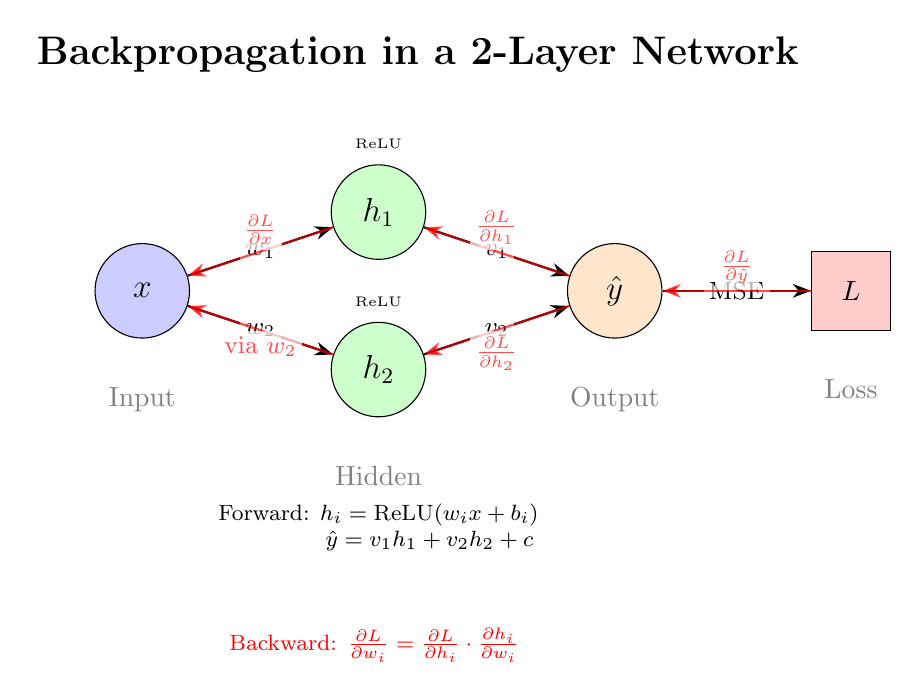
\begin{tikzpicture}[
    node distance=3cm,
    neuron/.style={circle, draw, fill=blue!20, minimum size=1.2cm, font=\large},
    hidden/.style={circle, draw, fill=green!20, minimum size=1.2cm, font=\large},
    output/.style={circle, draw, fill=orange!20, minimum size=1.2cm, font=\large},
    weight/.style={font=\small, midway, fill=white, inner sep=2pt},
    gradient/.style={font=\small, text=red, midway, fill=white, inner sep=2pt},
    layer/.style={font=\normalsize, text=gray},
    arrow/.style={-{Stealth[scale=1]}, thick},
    grad_arrow/.style={-{Stealth[scale=1]}, thick, red, opacity=0.7}
]

% Title
\node[font=\Large\bfseries] at (3.5, 3) {Backpropagation in a 2-Layer Network};

% Input layer
\node[neuron] (x) at (0, 0) {$x$};
\node[layer, below=0.5cm of x] {Input};

% Hidden layer
\node[hidden] (h1) at (3, 1) {$h_1$};
\node[hidden] (h2) at (3, -1) {$h_2$};
\node[layer, below=0.5cm of h2] {Hidden};

% Output layer
\node[output] (y) at (6, 0) {$\hat{y}$};
\node[layer, below=0.5cm of y] {Output};

% Loss
\node[draw, rectangle, fill=red!20, minimum size=1cm] (L) at (9, 0) {$L$};
\node[layer, below=0.5cm of L] {Loss};

% Forward connections
\draw[arrow] (x) -- (h1) node[weight] {$w_1$};
\draw[arrow] (x) -- (h2) node[weight] {$w_2$};
\draw[arrow] (h1) -- (y) node[weight] {$v_1$};
\draw[arrow] (h2) -- (y) node[weight] {$v_2$};
\draw[arrow] (y) -- (L) node[weight] {MSE};

% Backward gradients
\draw[grad_arrow] (L) -- (y) node[gradient, above] {$\frac{\partial L}{\partial \hat{y}}$};
\draw[grad_arrow] (y) -- (h1) node[gradient, above] {$\frac{\partial L}{\partial h_1}$};
\draw[grad_arrow] (y) -- (h2) node[gradient, below] {$\frac{\partial L}{\partial h_2}$};
\draw[grad_arrow] (h1) -- (x) node[gradient, above] {$\frac{\partial L}{\partial x}$};
\draw[grad_arrow] (h2) -- (x) node[gradient, below] {via $w_2$};

% Annotations
\node[align=left, font=\footnotesize, text=black] at (3, -3) {
Forward: $h_i = \text{ReLU}(w_i x + b_i)$\\
$\phantom{Forward: }\hat{y} = v_1 h_1 + v_2 h_2 + c$
};

\node[align=left, font=\footnotesize, text=red] at (3, -4.5) {
Backward: $\frac{\partial L}{\partial w_i} = \frac{\partial L}{\partial h_i} \cdot \frac{\partial h_i}{\partial w_i}$
};

% ReLU indicators
\node[font=\tiny, above=2pt of h1] {ReLU};
\node[font=\tiny, above=2pt of h2] {ReLU};

\end{tikzpicture}
\end{document}